\documentclass{article}
\usepackage[utf8x]{inputenc}
\usepackage{pgfplots}

\begin{document}

\section{Grafice de funcții}

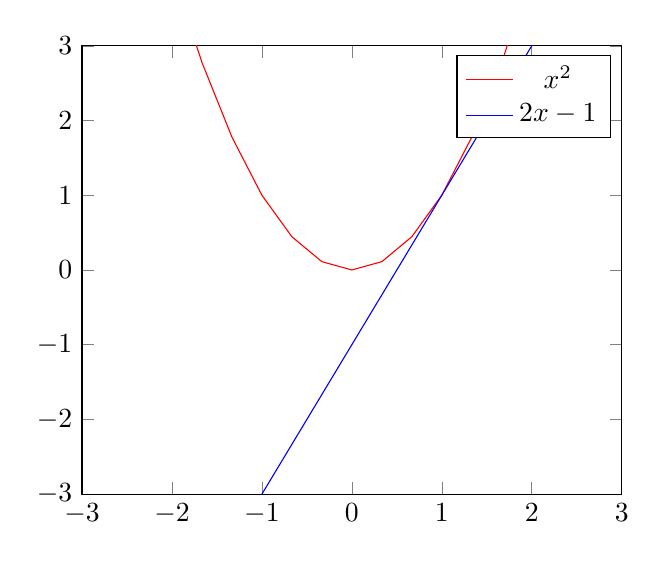
\begin{tikzpicture}
\begin{axis}[xtick={-3,-2,...,3}, ytick={-3,-2,...,3},xmin=-3, xmax=3, ymin=-3, ymax=3]
  \addplot[domain=-3:5,color=red]{x^2};
    \addlegendentry{$x^2$}
  \addplot[domain=-3:5,color=blue]{2*x-1};
    \addlegendentry{$2x-1$}
\end{axis}
\end{tikzpicture}

\textbf{1 Exercițiu:} adăugați graficul funcției $x^3$.

\newpage

\section{Configurarea axelor}

\pgfplotsset{my style/.append style={axis x line=middle, axis y line=middle, xlabel={$x$}, ylabel={$y$}, axis equal }}

\begin{tikzpicture}
\begin{axis}[my style, xtick={-3,-2,...,3}, ytick={-3,-2,...,3},xmin=-3, xmax=3, ymin=-3, ymax=3]
  \addplot[domain=-3:5]{-abs(x-1)+3};
  \addlegendentry{$-|x-1|+3$}
\end{axis}
\end{tikzpicture}

\newpage

\section{Funcții discontinue}

\begin{tikzpicture}
\begin{axis}[my style]
  \addplot[domain=-7:1] {-x-2};
  \addplot[domain=1:7] {x};
  \addplot[mark=*] coordinates {(1,-3)};
  \addplot[mark=*,fill=white] coordinates {(1,1)};
\end{axis}
\end{tikzpicture}

\end{document}